\documentclass{standalone}
\usepackage{tikz}
\begin{document}
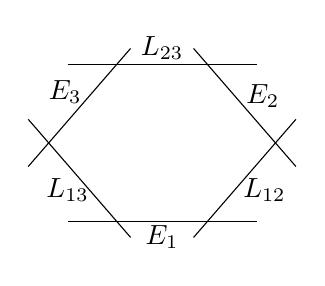
\begin{tikzpicture}  
\draw (-1.2,-1) -- (1.2,-1); % E_1
\draw (0.4,-1.2) -- (1.7,0.3); % L_12
\draw (-0.4,-1.2) -- (-1.7,0.3); % L_13
\draw (0.4,1.2) -- (1.7,-0.3);
\draw (-0.4,1.2) -- (-1.7,-0.3);
\draw (-1.2,1) -- (1.2, 1); % L_23

\node at (0,-1.2) {$E_1$};
\node at (1.3,-0.6) {$L_{12}$};
\node at (-1.2,-0.6) {$L_{13}$};
\node at (1.28, 0.6) {$E_2$};
\node at (-1.23, 0.65) {$E_3$};
\node at (0,1.2) {$L_{23}$};
\end{tikzpicture}

\end{document}